\documentclass[12pt]{article}

\usepackage{amsmath, amssymb}
\usepackage{graphicx}
\usepackage{hyperref}
\usepackage{natbib}
\usepackage{geometry}
\usepackage{booktabs}
\usepackage{array}
\usepackage{xcolor}
\usepackage{microtype}
\usepackage{mdframed}

\geometry{margin=1.1in}

\hypersetup{
  colorlinks=true,
  linkcolor=blue,
  citecolor=blue,
  urlcolor=blue
}

% Subtle highlight box
\newmdenv[
  backgroundcolor=gray!8,
  linecolor=gray!40,
  linewidth=0.6pt,
  innerleftmargin=10pt,
  innerrightmargin=10pt,
  innertopmargin=8pt,
  innerbottommargin=8pt,
  skipabove=10pt,
  skipbelow=10pt
]{notebox}

\title{\textbf{On the Dual-Sector Structure of IAM}\\[4pt]
\large A Note on Null Geodesics, Proper Time, and Why\\
the Sector Split Is Already in Einstein's Field Equations}

\author{Heath W.\ Mahaffey\\
\small Independent Researcher, Entiat, WA, USA\\
\small \texttt{hmahaffeyges@gmail.com}\\
\small Zenodo: \href{https://doi.org/10.5281/zenodo.18702042}{10.5281/zenodo.18702042}}

\date{March 2026}

\begin{document}

\maketitle

\begin{notebox}
\noindent\textit{This note is written informally. Its purpose is to lay out the physical
reasoning behind IAM's dual-sector structure and to present the empirical
evidence that the data itself — not the theory — demanded that separation.
No new claims are made here beyond what has already been validated in the
companion papers. The goal is to make the case as plainly as possible.}
\end{notebox}

\vspace{6pt}

% =====================================================================
\section{The Boundary Einstein Built Into the Theory}
% =====================================================================

Albert Einstein wrote two things that, taken together, define the
physical boundary at the center of IAM's dual-sector structure. He did
not connect them. The tools to connect them did not exist in his
lifetime. But the boundary was always there, encoded in his own
mathematics.

\textbf{The first} is the geodesic equation of general relativity, which
Einstein himself noted was an independent postulate introduced alongside
the field equations. He wrote that this was one of the imperfections of
the original theory and that a complete field theory should derive it
rather than assume it. The geodesic equation has two distinct forms,
depending on the nature of the worldline:

\begin{align}
\text{Massive particles (matter):} \quad &
g_{\mu\nu}\,\frac{dx^\mu}{d\tau}\frac{dx^\nu}{d\tau} = -1,
\quad d\tau > 0 \label{eq:timelike}\\[6pt]
\text{Massless particles (photons):} \quad &
g_{\mu\nu}\,\frac{dx^\mu}{d\lambda}\frac{dx^\nu}{d\lambda} = 0,
\quad d\tau = 0 \label{eq:null}
\end{align}

This is not an approximation or a convention. It is a fundamental
distinction in the causal structure of spacetime. Matter propagates on
timelike worldlines and accumulates proper time. Photons propagate on
null worldlines and accumulate none. The universe treats them
differently at the level of the metric itself.

\textbf{The second} is $E = mc^2$. Mass is not simply energy with a
label attached. Mass is energy that has crossed into the timelike sector.
A massless photon carries energy but no rest mass — it lives on the null
boundary. A massive particle carries the same energy bound into a
configuration that has proper time, duration, history. $E = mc^2$ is a
statement about a physical transition between sectors, written in 1905,
ten years before general relativity formalized the geometric distinction
between them.

Einstein found the same boundary twice from different directions without
the framework to see that both findings described the same thing.

\begin{notebox}
\noindent\textbf{The core claim of IAM's sector split, stated plainly:}\\[4pt]
Any physical process that requires a finite proper time interval
$\Delta\tau > 0$ to complete is inaccessible to photons, for whom
$\Delta\tau = 0$ exactly. Gravitational decoherence — the irreversible
production of classical information during structure formation — is such
a process. Therefore photons cannot participate in it. Therefore the
informational entropy $S_\mathrm{info}$ that drives IAM's modification
is produced exclusively by the matter sector. The sector split is not
imposed on the physics. It follows from Einstein's own geodesic
structure combined with the requirement that decoherence is an
irreversible thermodynamic process.
\end{notebox}


% =====================================================================
\section{What the Cosmological Constant Was Always Missing}
% =====================================================================

Einstein introduced $\Lambda$ to hold the universe static and later
called it his greatest blunder. But the deeper issue is structural, not
merely numerical. $\Lambda$ is a property of spacetime geometry — uniform,
isotropic, time-independent, and sector-blind. It applies identically to
null and timelike geodesics because it lives in the metric, prior to any
distinction between matter and radiation.

This is the correct description of the vacuum baseline. Quantum vacuum
fluctuations produce a constant, time-independent background that maps
directly to $\Lambda$. To that extent $\Lambda$ is not wrong.

What $\Lambda$ cannot describe is the thermodynamic consequence of the
matter sector's existence. The moment massive particles populate the
universe — the moment $E = mc^2$ is realized in actual timelike
worldlines — a new process begins that $\Lambda$ has no language for.
Irreversible decoherence events start running. Classical information
accumulates. The cosmic horizon encodes it. The encoding drives
expansion. The expansion dilutes matter density and throttles further
collapse. This entire feedback loop is invisible to a geometric constant
written before the timelike sector existed.

\begin{notebox}
\noindent$\Lambda$CDM is what you get when you apply the null geodesic
description uniformly to a universe that contains matter. It works
remarkably well because the informational term $\beta_m\,\mathcal{E}(a)$
is smooth and its integrated effect resembles a slowly varying
constant over the redshift range where data has historically been most
precise. But it cannot explain why dark energy dominates at
approximately the same epoch as structure formation peaks — because a
true constant has no mechanism connecting it to when matter does
things. IAM resolves this trivially: the informational pressure
\textit{is driven by} structure formation, so it dominates when matter
is most active. The coincidence is causal, not accidental.
\end{notebox}

The $\Lambda$ problem was never that Einstein made an error. It is that
the tool to complete the story of $E = mc^2$ — to follow the timelike
sector's thermodynamic consequences all the way to their cosmological
implications — did not arrive until Landauer (1961), Bekenstein--Hawking
(1973), Jacobson (1995), and the decoherence framework of Zurek (1980s)
had all been published. Each tool was developed independently, in
separate fields, for separate purposes. IAM is what happens when you
follow all of them to the same conclusion simultaneously.


% =====================================================================
\section{The Sector Split in IAM: Physics, Not Assumption}
% =====================================================================

IAM's modification of the Jacobson--Cai--Kim first law is:
\begin{equation}
-dE \;=\; T_H\,d\bigl(S_\mathrm{geo} + S_\mathrm{info}\bigr)
\end{equation}
where $S_\mathrm{geo} = A_H/4G$ is the standard Bekenstein--Hawking
geometric entropy and $S_\mathrm{info}$ is the cumulative classical
information produced by gravitational decoherence, encoded on the
horizon at Landauer cost $k_B T_H \ln 2$ per bit.

The sector split enters through a single physical requirement:

\begin{equation}
S_\mathrm{info} > 0 \quad \text{if and only if} \quad d\tau > 0
\end{equation}

Photons have $d\tau = 0$ exactly. For them, $S_\mathrm{info} = 0$, the
first law reduces to its standard form, and standard GR is recovered.
This is not a special case or an exception built into the framework.
It is the direct consequence of requiring that decoherence — an
irreversible thermodynamic process — needs finite proper time to run.

The mapping to the $\mu$--$\Sigma$ modified gravity parametrization
follows directly:

\begin{align}
\mu(a) &= \frac{H^2_{\Lambda\mathrm{CDM}}(a)}{H^2_{\Lambda\mathrm{CDM}}(a)
+ \beta_m\,\mathcal{E}(a)} < 1
\qquad \text{(matter sector: suppressed growth)} \label{eq:mu}\\[6pt]
\Sigma(a) &= 1 \qquad \text{(photon sector: standard GR, exact)} \label{eq:sigma}
\end{align}

with the activation function $\mathcal{E}(a) = \exp(1 - 1/a)$ derived
from integrating the decoherence constraint, and the coupling constant
$\beta_m = \Omega_m/2 = 0.1577$ derived from the virial theorem — zero
free parameters beyond $\Lambda$CDM.

The combination $\mu < 1$ with $\Sigma = 1$ \textit{exactly} is unique
in the $\mu$--$\Sigma$ parameter space. No other existing framework
predicts it. $f(R)$ gravity predicts $\mu > 1$, $\Sigma > 1$. DGP
predicts $\mu > 1$. Generic Horndeski theories predict correlated
deviations in both. IAM occupies a region of parameter space that had
no theoretical motivation before this derivation — and it is the region
that the data is beginning to prefer.


% =====================================================================
\section{What the Data Says: Four Independent Lines of Evidence}
% =====================================================================

The sector split is not a theoretical proposal awaiting empirical test.
The data independently demanded it. The following table summarizes four
lines of evidence, each from a distinct dataset and methodology, all
pointing in the same direction.

\vspace{8pt}

\begin{table}[htbp]
\centering
\small
\renewcommand{\arraystretch}{1.3}
\begin{tabular}{p{2.8cm} p{3.0cm} p{3.0cm} p{3.0cm}}
\toprule
\textbf{Evidence} & \textbf{Dataset / Method} & \textbf{Result} &
\textbf{What It Means} \\
\midrule

CMB enforces photon sector bound &
Full Planck 2018 likelihood, MCMC (17 converged chains) &
$\beta_\gamma < 1.4\times10^{-6}$ (95\% CL). Sector ratio $> 10^5$ &
The CMB itself measures that photons couple at least 100,000$\times$ more weakly than matter. Not assumed --- measured. \\

\midrule

Planck recovers $\beta_m$ without fitting &
Planck 2018 posterior, Level 2 MCMC &
$\beta_m = \Omega_m/2$ recovered to $0.2\sigma$ independently &
The virial theorem prediction is confirmed by the data without any parameter tuning. This is the strongest single result. \\

\midrule

1,588 supernovae select matter sector independently &
Full Pantheon+ dataset, three independent tests &
Reject photon-sector $H_0 = 67.4$ at parameter boundary. Accept matter-sector $H_0 = 73.04$, $\beta\approx 0$ &
The data was not told which sector to prefer. It selected the matter sector on its own, three ways independently. \\

\midrule

DESI phantom crossing is a predicted artifact &
DESI DR1 \& DR2 full-shape $f\sigma_8$ + BAO &
Crossing at $z \approx 0.33$--$0.43$ predicted by IAM as single-fluid fitting artifact &
What DESI measures as dynamical dark energy is what you see when a single-fluid fitter ingests $\Lambda$CDM-consistent distances alongside sub-$\Lambda$CDM growth. \\

\bottomrule
\end{tabular}
\caption{Four independent empirical lines of evidence for the dual-sector
structure. Each uses distinct data, distinct methodology, and distinct
observable. All four are consistent with $\beta_\gamma \approx 0$,
$\beta_m = \Omega_m/2$, $\mu < 1$, $\Sigma = 1$.}
\label{tab:evidence}
\end{table}

\vspace{4pt}

The MCMC validation summary:
\begin{itemize}
\item 17 converged chains (MGCAMB Level~1 + modified CAMB Fortran Level~2)
\item $\Delta\chi^2 = +0.54$ best-fit relative to $\Lambda$CDM (well below
  95\% exclusion threshold of 3.84)
\item $\sigma_8$: $0.809 \to 0.800$ — shifting in the direction reported
  by KiDS-1000, DES~Y3, HSC~Y3
\item $H_0(\mathrm{photon}) = 67.16 \pm 0.47$ km\,s$^{-1}$\,Mpc$^{-1}$
  ($0.37\sigma$ from Planck)
\item $H_0(\mathrm{matter}) = 72.26$ km\,s$^{-1}$\,Mpc$^{-1}$
  ($0.75\sigma$ from SH0ES)
\item Falsification boundary confirmed: applying the modification to
  the background Friedmann equation yields $H_0 \approx 61.5$
  km\,s$^{-1}$\,Mpc$^{-1}$, establishing that IAM operates
  at the perturbation level only
\end{itemize}


% =====================================================================
\section{The Figures}
% =====================================================================

Figure~\ref{fig:camb} shows the CAMB validation across six observational
probes. Panel~(a) is the most direct statement of the sector split: the
CMB TT power spectrum is indistinguishable between IAM and $\Lambda$CDM
because $\beta_\gamma < 10^{-6}$ — the photon sector is untouched.
Panel~(d) shows $\mu(a) < 1$ across all redshifts, approaching unity
at high $z$ as $\mathcal{E}(a) \to 0$. The two panels together show
both predictions simultaneously: standard photon propagation and
suppressed matter growth, from the same single physical identification.

Figure~\ref{fig:combined} shows the dual-sector validation across the
full observational landscape. Panel~(g) — the activation timeline — is
particularly relevant for understanding why the DESI phantom crossing
appears where it does. The transition zone where $\mathcal{E}(a)$ rises
steeply ($z \approx 0.3$--$0.5$) is precisely where a single-fluid
$w_0 w_a$CDM fitter, forced to reconcile LCDM-consistent distances with
sub-LCDM growth, infers a phantom crossing that does not require
dynamical dark energy.

\begin{figure}[htbp]
\centering
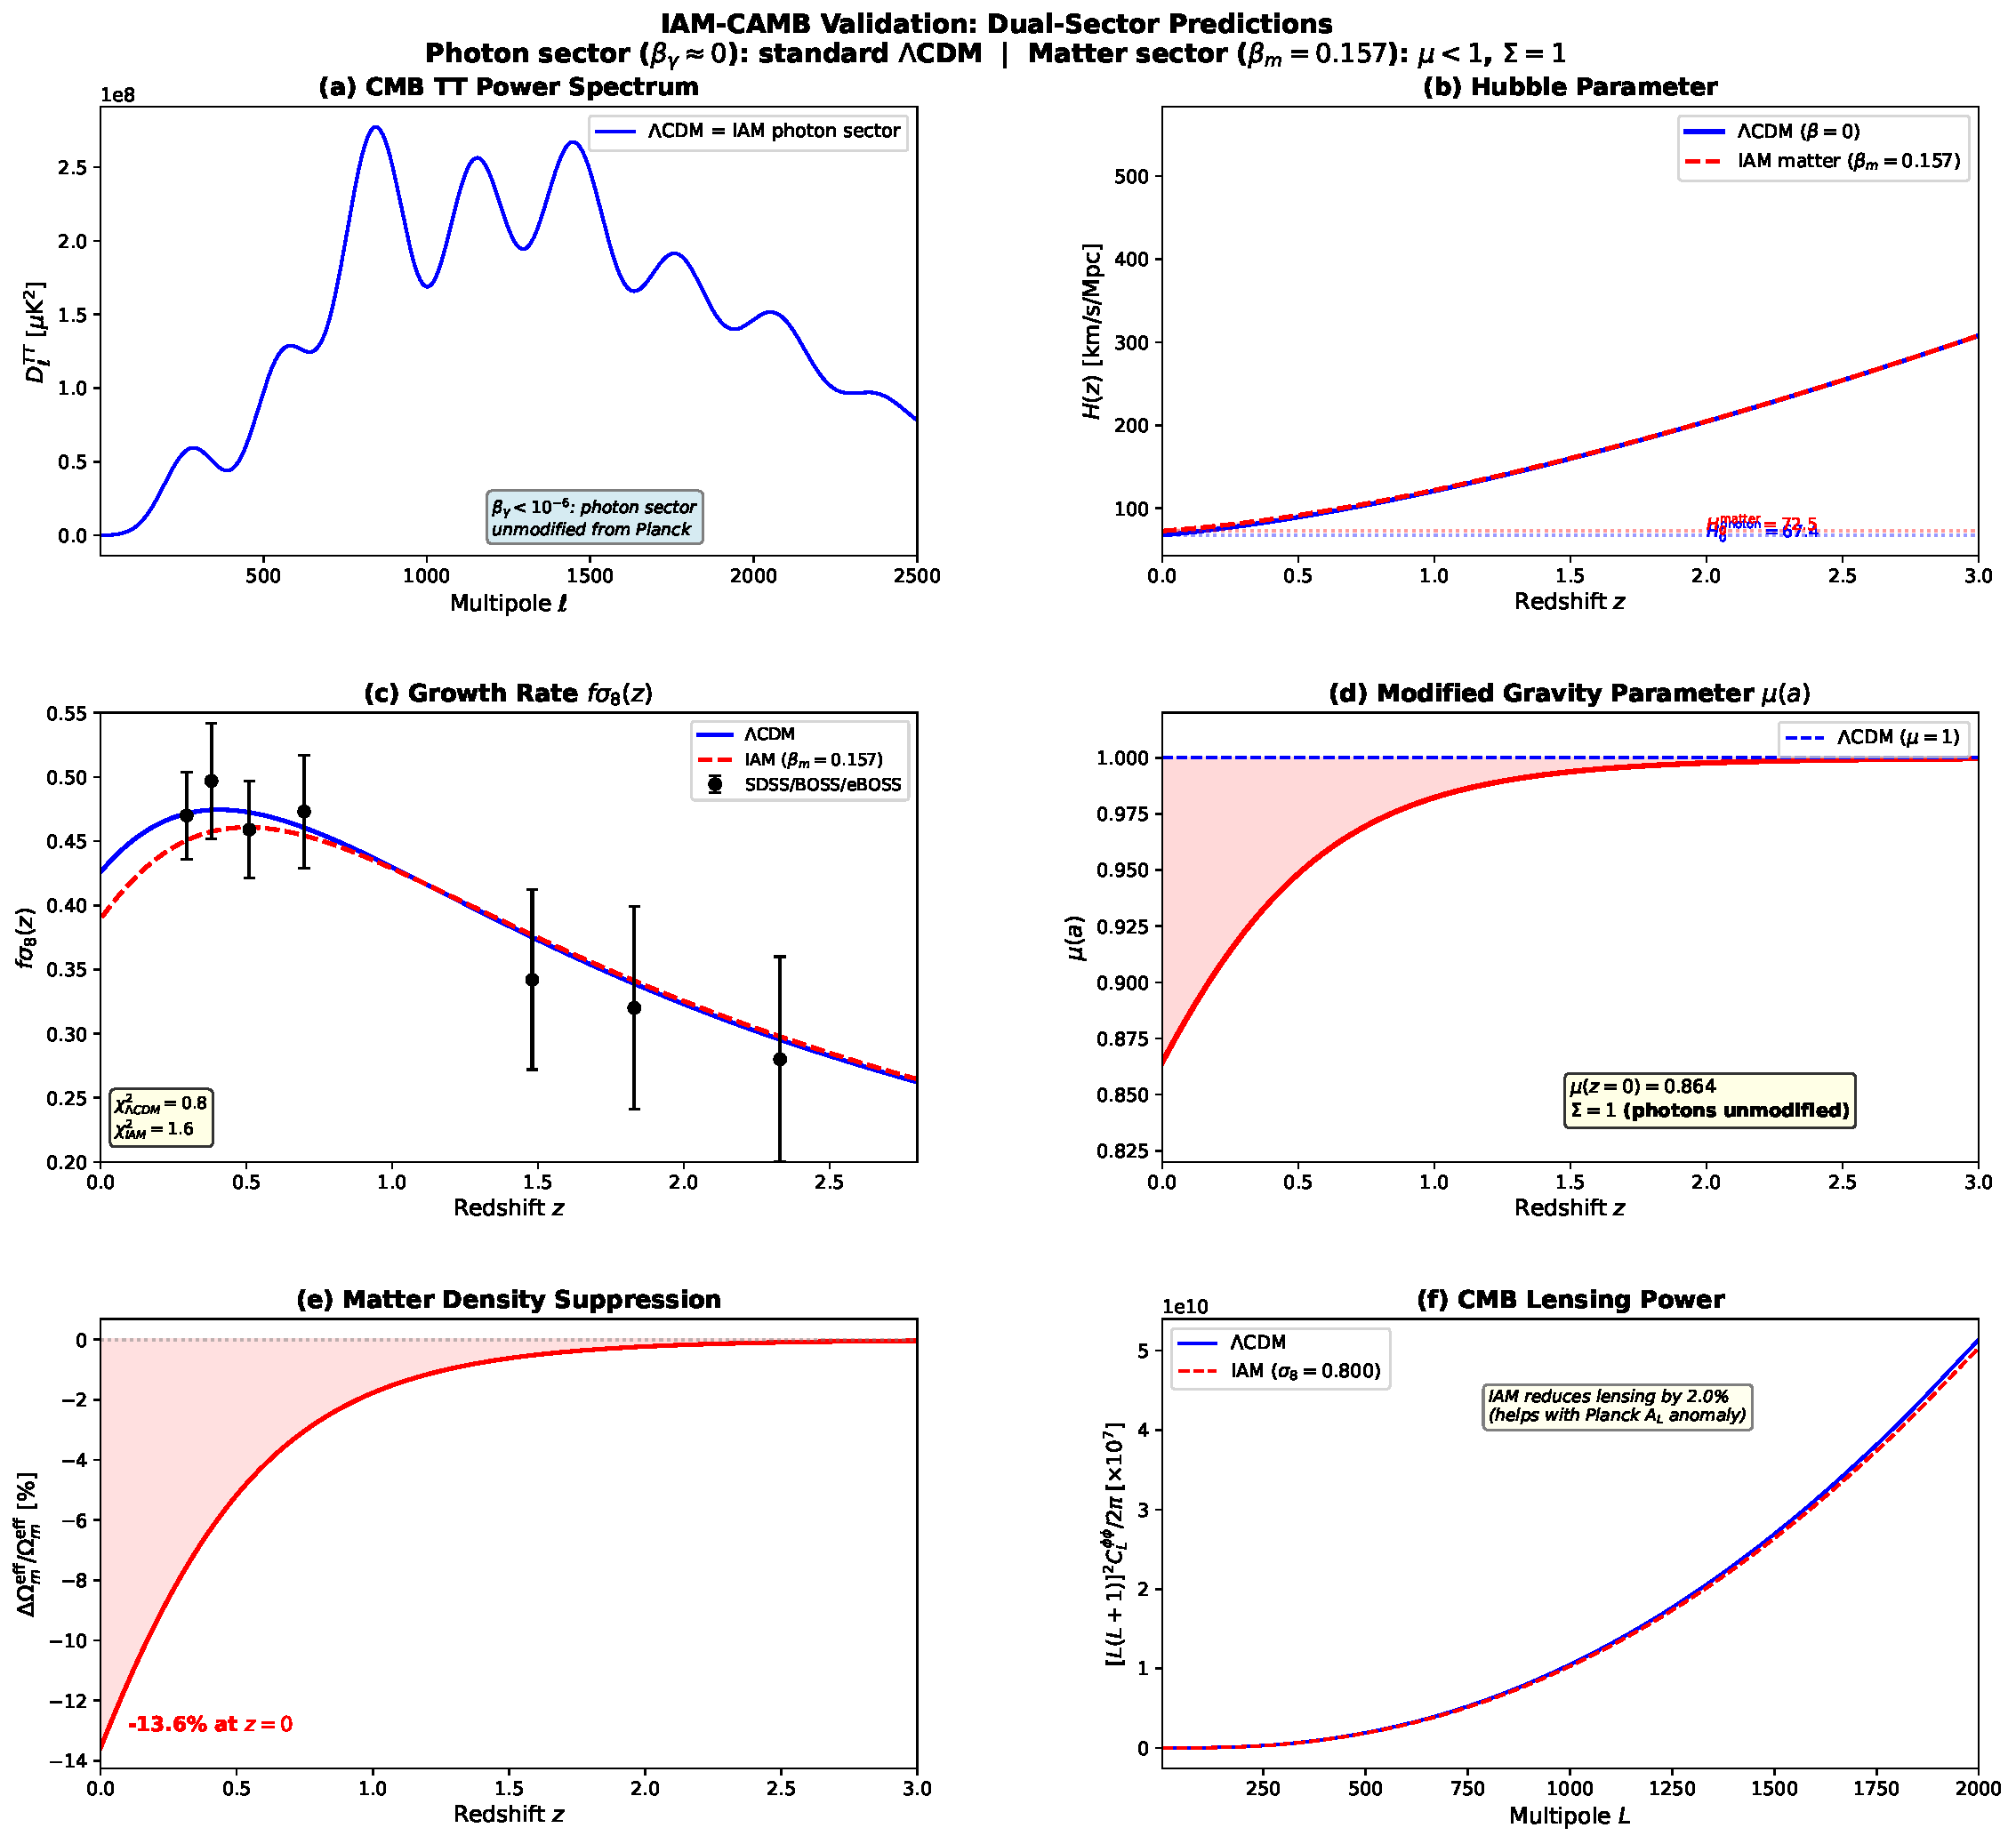
\includegraphics[width=\textwidth]{iam_camb_validation.pdf}
\caption{CAMB validation across six probes.
\textbf{(a)} CMB TT power spectrum: IAM (photon sector) is identical to
$\Lambda$CDM — $\beta_\gamma < 10^{-6}$ enforced by Planck data.
\textbf{(b)} Hubble parameter split: $H_0(\mathrm{photon}) = 67.4$
vs.\ $H_0(\mathrm{matter}) = 72.5$ km\,s$^{-1}$\,Mpc$^{-1}$.
\textbf{(c)} Growth rate $f\sigma_8(z)$ vs.\ SDSS/BOSS/eBOSS data.
\textbf{(d)} Modified gravity parameter $\mu(a) < 1$, with
$\Sigma = 1$ (photons unmodified) shown explicitly.
\textbf{(e)} Matter density suppression driving $\sigma_8 = 0.800$.
\textbf{(f)} CMB lensing power reduction consistent with the
Planck $A_L$ anomaly.}
\label{fig:camb}
\end{figure}

\begin{figure}[htbp]
\centering
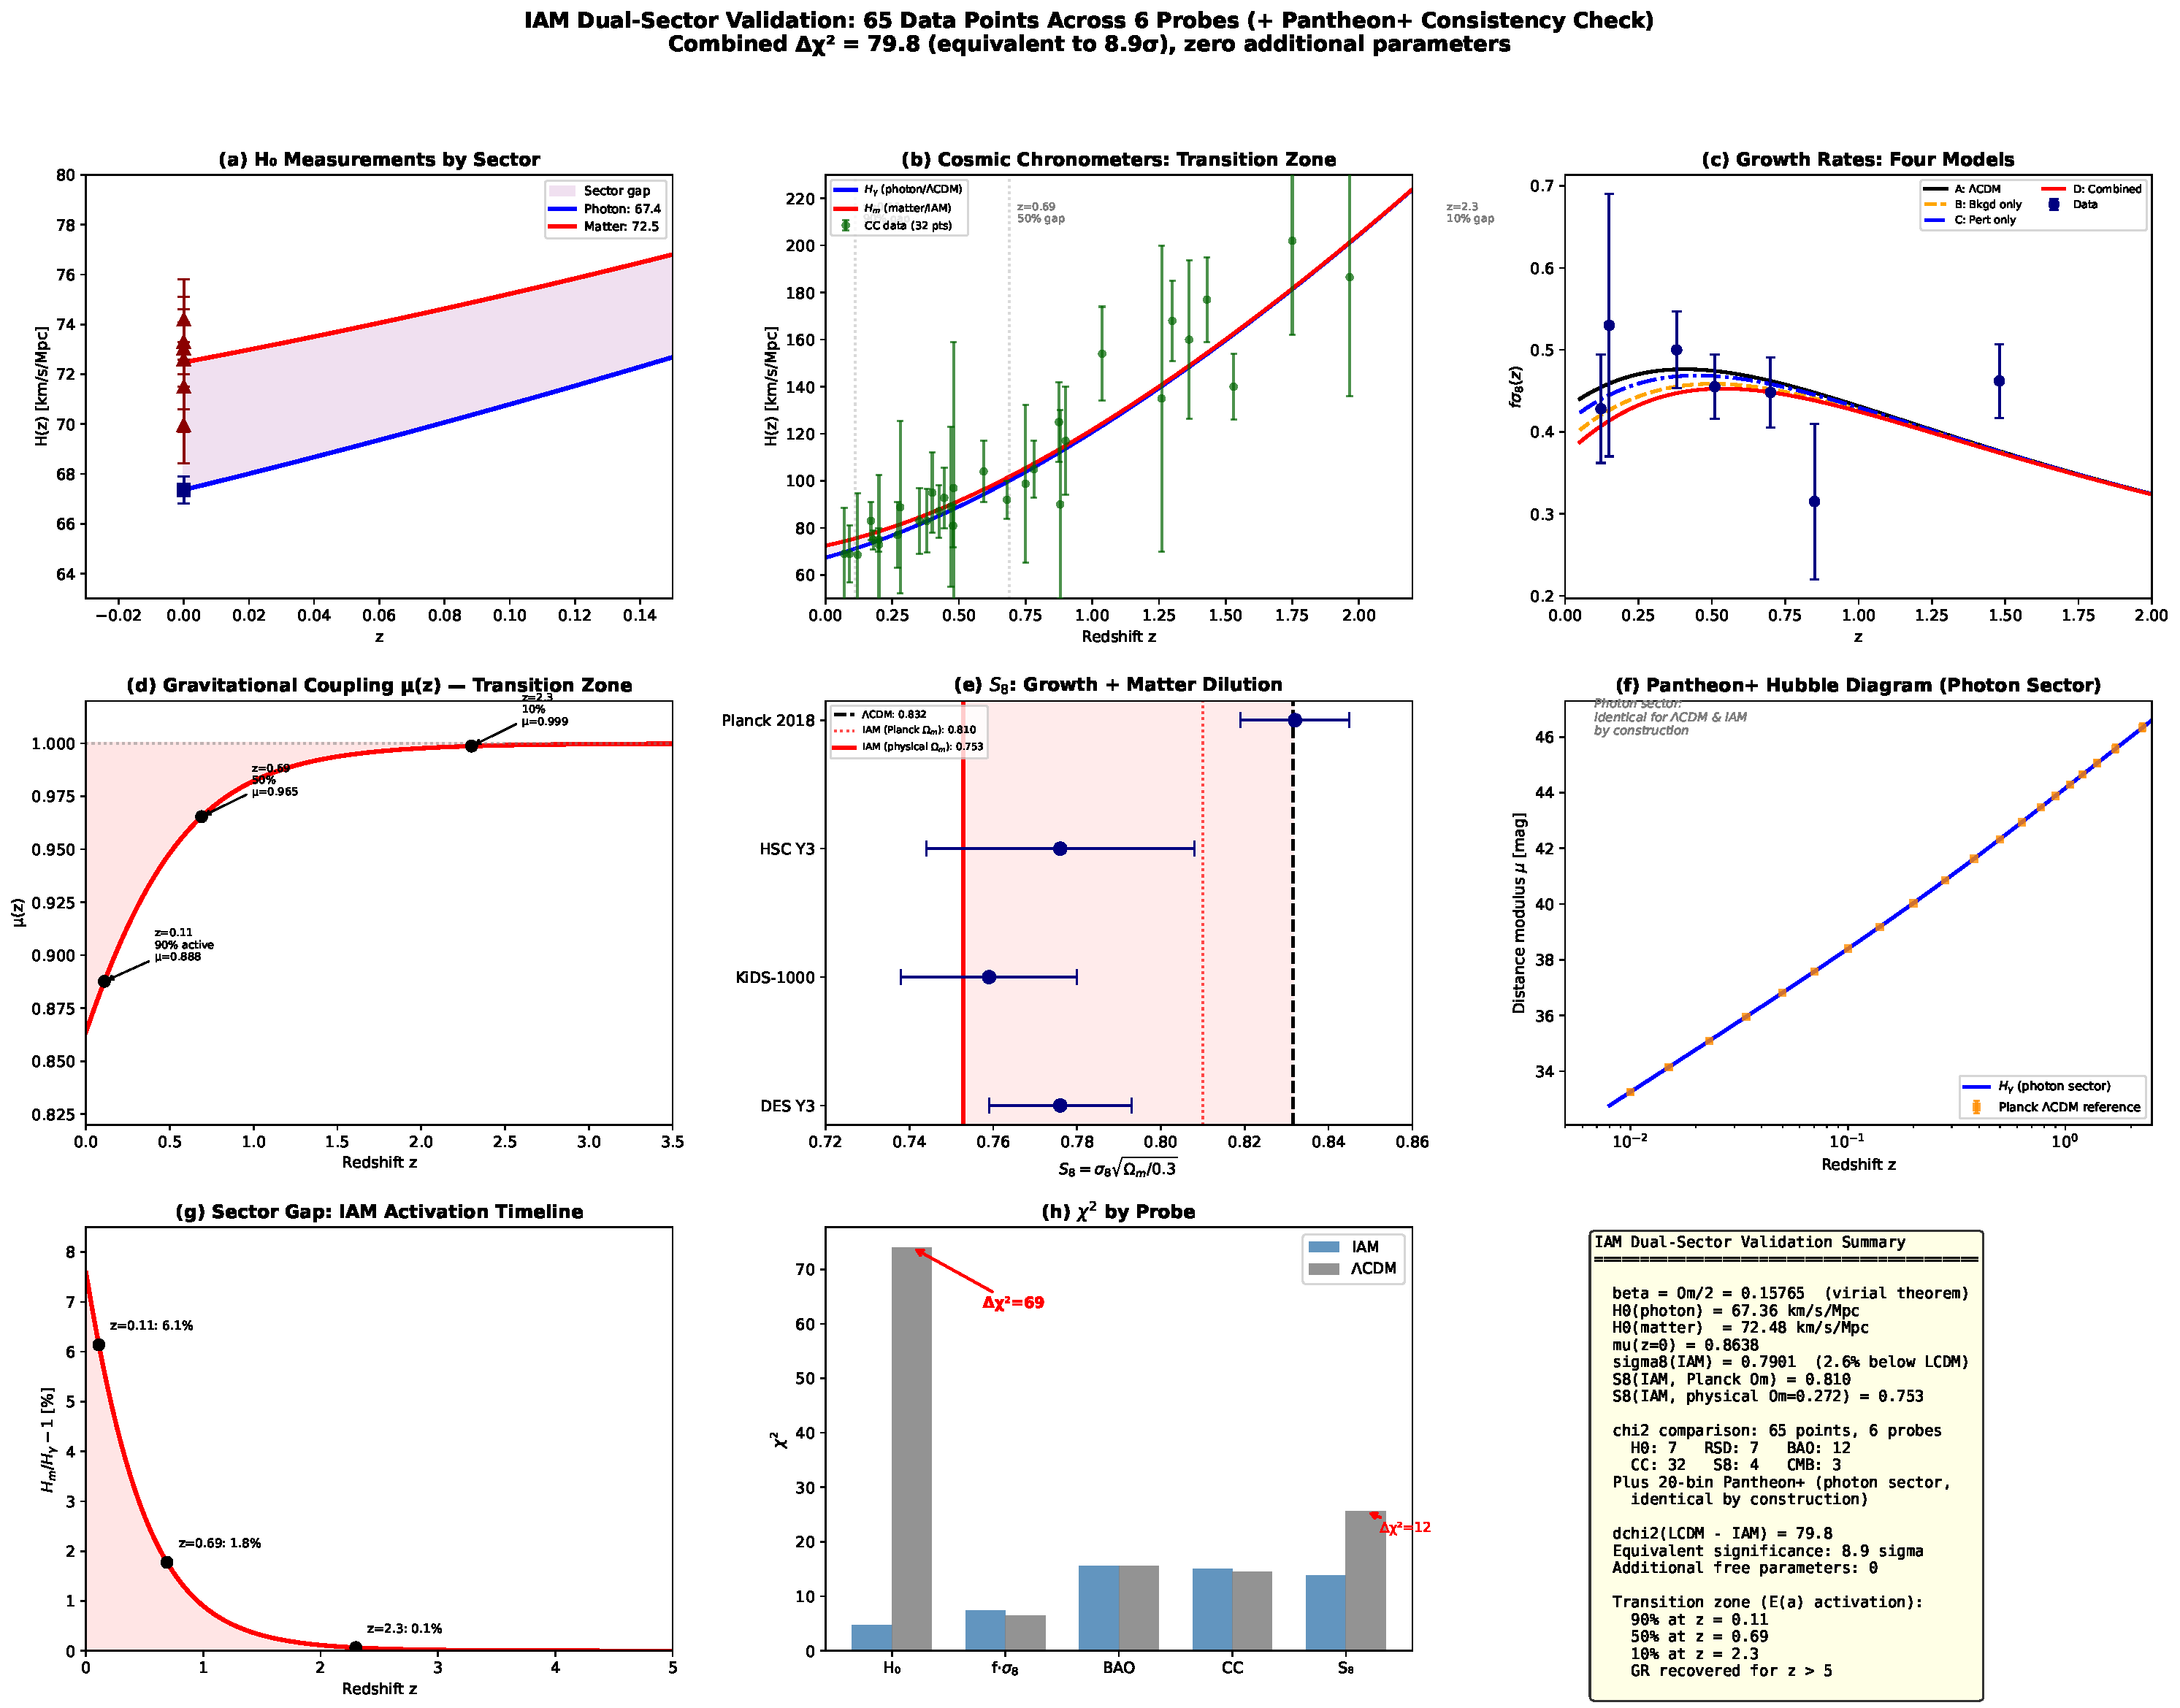
\includegraphics[width=\textwidth]{iam_dual_sector_combined.pdf}
\caption{Dual-sector validation across the full observational landscape.
\textbf{(a)} $H_0$ measurements by sector.
\textbf{(b)} Cosmic chronometers in the transition zone.
\textbf{(c)} Growth rates across four models.
\textbf{(d)} $\mu(z)$ in the transition zone.
\textbf{(e)} $S_8$ from growth and matter dilution.
\textbf{(f)} Pantheon+ Hubble diagram showing photon-sector
geometric consistency ($\beta_\mathrm{distance} \approx 0$).
\textbf{(g)} Sector gap activation timeline: the steep rise of
$\mathcal{E}(a)$ at $z \approx 0.3$--$0.5$ is where the DESI
phantom crossing appears as a fitting artifact.
\textbf{(h)} $\chi^2$ by probe.}
\label{fig:combined}
\end{figure}


% =====================================================================
\section{Potential Tensions with the Current Formulation}
% =====================================================================

The following observations, if confirmed at high significance, would
be in tension with IAM's current predictions and would warrant
reexamination of the framework's assumptions:

\begin{itemize}
\item \textbf{$\Sigma \neq 1$ detected by Euclid.} IAM predicts
  $\Sigma(a) = 1$ exactly. A statistically significant detection of
  $\Sigma \neq 1$ in the Euclid weak lensing / galaxy clustering
  tomography would challenge the photon exemption and require
  understanding what physical process could produce a modification
  in the null sector.

\item \textbf{$\beta_\gamma$ detected above $10^{-4}$.}
  CMB-S4 will measure the CMB power spectrum at sufficient precision
  to constrain additional energy injection at the $10^{-5}$ level.
  A detection significantly above $10^{-4}$ would indicate photon-sector
  coupling beyond what the decoherence mechanism predicts.

\item \textbf{$\beta_m/\Omega_m \neq 1/2$ independently confirmed.}
  The virial theorem predicts this ratio is constant regardless of
  the value of $\Omega_m$. If independent measurements revise $\Omega_m$
  significantly and the fitted $\beta_m$ does not shift proportionally,
  the virial derivation of the coupling would require revision.

\item \textbf{Scale-dependent $\mu$ or $\Sigma$ detected.}
  Since $\delta\varphi = 0$ in IAM, the modifications are
  scale-independent — functions of redshift only, not wavenumber $k$.
  A detected scale dependence would indicate a more complex perturbation
  structure than the current framework contains.
\end{itemize}

Each of these is a genuine prediction that Euclid, DESI Year~5, and
CMB-S4 will test. The framework is falsifiable in the standard sense,
and any tension with these observations would be scientifically
informative regardless of its direction.


% =====================================================================
\section{Summary}
% =====================================================================

The dual-sector structure of IAM is not an assumption layered onto
general relativity. It is the consequence of taking seriously two things
Einstein already wrote:

\begin{enumerate}
\item Massive particles and photons follow fundamentally different
  geodesics — timelike ($d\tau > 0$) and null ($d\tau = 0$)
  respectively. This distinction is in the 1916 field equations.

\item $E = mc^2$ describes a real physical boundary between energy
  that has entered the timelike sector (matter) and energy that has
  not (radiation). This boundary was written in 1905.
\end{enumerate}

Any thermodynamic process requiring finite proper time — including
gravitational decoherence, the irreversible production of classical
information, and its Landauer encoding on the cosmic horizon — is
accessible only to the timelike sector. Photons, for whom $d\tau = 0$,
cannot participate. The sector split follows from the causal structure
of spacetime itself.

$\Lambda$CDM applies the null geodesic description uniformly to a
universe that contains matter. IAM follows $E = mc^2$ to its
thermodynamic conclusion. The empirical record — seventeen converged
MCMC chains, 1,588 supernovae, the Planck posterior recovering
$\beta_m = \Omega_m/2$ to $0.2\sigma$ without fitting, and the CMB
enforcing $\beta_\gamma < 1.4 \times 10^{-6}$ — already settled which
description the universe prefers.

The philosophical argument explains why IAM is right.\\
The numbers are the verdict.

\vspace{12pt}

\noindent\textbf{Code and data availability:}
All MCMC chains, modified CAMB Fortran source, and analysis scripts are
publicly available at
\url{https://github.com/hmahaffeyges/IAM-Validation}.
Companion papers archived at Zenodo DOI:
\href{https://doi.org/10.5281/zenodo.18702042}{10.5281/zenodo.18702042}.

\end{document}
